\documentclass{beamer}

\usepackage[english]{babel}
\usepackage{amssymb,amsmath,amsthm,animate,epsfig,multimedia,pstricks,times}

\def\black{\color{black}}
\def\blue{\color{blue}}

\newcommand{\R}{{\mathbb R}}
\newcommand{\vol}{\mathcal{L}^d}
\newcommand{\dH}[1]{\;{\rm d}{\cal H}^{#1}} % Hausdorff measure
\newcommand{\dL}[1]{\;{\rm d}{\cal L}^{#1}} % Lebesgue measure
\newcommand{\bigchi}{\ensuremath{\mathrm{\mathcal{X}}}}
\newcommand{\charfcn}[1]{\bigchi_{#1}} % characteristic function
\newcommand{\Vh}{\underline{V}(\Gamma^m)}
\newcommand{\Wh}{W(\Gamma^m)}
\newcommand{\Vht}{\underline{V}(\Gamma^h(t))}
\newcommand{\Wht}{W(\Gamma^h(t))}
\newcommand{\uspace}{\mathbb{U}}
\newcommand{\pspace}{\mathbb{P}}
\newcommand{\kspace}{\mathbb{K}}
\newcommand{\xspace}{\mathbb{X}}
\newcommand{\sigmaO}{o}
\newcommand{\nabs}{\nabla_{\!s}}
\newcommand{\id}{\rm id}
\newcommand{\ddt}{\frac{\rm d}{{\rm d}t}}
\newcommand{\NbulkT}{\vec{N}_{\Gamma,\Omega}^T}
\newcommand{\Nbulk}{\vec{N}_{\Gamma,\Omega}}
\newcommand{\unitn}{\vec{\rm n}}
\newcommand{\mat}[1]{\underline{\underline{#1}}\rule{0pt}{0pt}}

\title{Fitted ALE scheme for Two-Phase Navier--Stokes Flow}
\author{\underline{Marco Agnese} and Robert N\"urnberg}
\institute[]{Imperial College London}
\date[]{$8^{th}$ September 2016}

\begin{document}

\begin{frame}
\titlepage
\end{frame}

\begin{frame}
\frametitle{Problem setting}

Domain $\Omega$ in the 2-dimensional case.

\begin{figure}
\begin{center}
\unitlength15mm
\psset{unit=\unitlength,linewidth=1pt}
\begin{picture}(4,4)(0,0)
\psline(0,0)(4,0)(4,4)(0,4)(0,0)
\psellipse(2,2)(1,1)
\psline{->}(3,2)(3.5,2)
\put(3.25,1.75){$\vec\nu$}
\put(1.75,0.75){{$\Gamma(t)$}}
\put(1.75,2){{$\Omega_-(t)$}}
\put(0.5,3.25){{$\Omega_+(t)$}}
\end{picture}
\end{center}
\end{figure}

\end{frame}

\begin{frame}
\frametitle{Governing equations}

\begin{itemize}
\item Bulk equations
\begin{subequations}
\begin{alignat*}{2}
\rho\,(\vec u_t + (\vec u \,.\,\nabla)\,\vec u)
- \nabla\,.\,\mat\sigma & = \vec f = \rho\,\vec f_1 + \vec f_2 \qquad &&
\mbox{in } \Omega_\pm(t)\,, \\
\nabla\,.\,\vec u & = 0 \qquad &&\mbox{in } \Omega_\pm(t)\,,
\end{alignat*}
\end{subequations}
where
\begin{equation*}
\mat\sigma = \mu \,(\nabla\,\vec u + (\nabla\,\vec u)^T) - p\,\mat\id\
= 2\,\mu\, \mat D(\vec u)-p\,\mat\id\,.
\end{equation*}

\item Interface equations
\begin{subequations}
\begin{alignat*}{2}
[\vec u]_-^+ & = \vec 0 \qquad &&\mbox{on } \Gamma(t)\,, \\
[\mat\sigma\,\vec \nu]_-^+ & = -\gamma\,\varkappa\,\vec\nu \qquad
&&\mbox{on } \Gamma(t)\,, \\
\vec{\mathcal{V}}\,.\,\vec\nu &= \vec u\,.\,\vec \nu \qquad
&&\mbox{on } \Gamma(t)\,.
\end{alignat*}
\end{subequations}

\item To close the system, we prescribe the initial data $\Gamma(0) = \Gamma_0$,
the initial velocity $\vec u_0$ and some boundary condition for $\vec u$ on
$\partial \Omega$.
\end{itemize}
\end{frame}

\begin{frame}
\frametitle{Interface treatment}

\begin{itemize}
\item $\Gamma(t)$ is a sufficiently smooth evolving hypersurface without
boundary that is parameterized by $\vec x(\cdot,t):\Upsilon\to\R^d$, therefore
\begin{equation*}
\Gamma(t) = \vec x(\Upsilon,t)\,,
\end{equation*}
where $\Upsilon\subset \R^d$ is a given reference manifold.

\item It holds that
\begin{equation*}
\Delta_s\, \vec \id = \varkappa\, \vec\nu \qquad \mbox{on $\Gamma(t)$}\,,
\end{equation*}
where $\Delta_s = \nabs\,.\,\nabs$ is the Laplace-Beltrami operator on
$\Gamma(t)$ with $\nabs\,.\,$ and $\nabs$ denoting surface divergence and
surface gradient on $\Gamma(t)$.
\end{itemize}
\end{frame}

\begin{frame}
\frametitle{Arbitrary Lagrangian Eulerian approach}

\begin{itemize}

\item In the ALE approach, a prescribed flow drives the movement of the bulk
mesh vertices.

\item Let $h:\Omega_{\pm}(t)\times [0,T]\to \mathbb{R}$ be a function defined on
the Eulerian frame, the corresponding function on the ALE frame $\hat h$ is
defined as
\begin{equation*}
\hat h:\Upsilon_{\Omega_\pm}\times [0,T]\to \mathbb{R},\qquad
\hat h(\vec q,t)=h(\vec{x}(\vec q,t),t)
\end{equation*}
and it holds
\begin{equation*}
h_t =\left.h_t\right|_{\Upsilon_{\Omega_\pm}} -\vec{\mathcal{W}} \cdot \nabla h.
\end{equation*}

\item The movement of the bulk mesh is incorporated in the finite element
approximation therefore it avoids the repeated interpolation of the
velocity onto the bulk mesh.
\end{itemize}

\end{frame}

\begin{frame}
\frametitle{Weak formulation}

Using the function spaces
\begin{subequations}
\begin{align*}
\uspace &:= [H^1_0(\Omega)]^d\,,\qquad \pspace := L^2(\Omega) \qquad
\mbox{and} \\
\widehat\pspace &:= \{\eta\in\pspace : \int_\Omega\eta\dL{d}=0 \}\,,
\end{align*}
\end{subequations}
the Navier--Stokes weak formulation is
\begin{subequations}
\begin{align*}
& (\rho\,\left.\vec{u}_t\right|_{\Upsilon_{\Omega_\pm}}, \vec \xi)
+ (\rho\,(\vec u - \vec{\mathcal{W}})\,.\,\nabla\,
\vec u\,,\,\vec \xi) +2\left(\mu\,\mat D(\vec u), \mat D(
\vec \xi)\right) \nonumber \\
& - \left(p, \nabla\,.\,\vec \xi\right)
- \gamma\,\left\langle \varkappa\,\vec\nu, \vec\xi\right\rangle_{\Gamma(t)}
= \left(\vec f, \vec \xi\right)\quad \forall\ \vec\xi \in \uspace \,, \\
& \left(\nabla\,.\,\vec u, \varphi\right) = 0
\quad \forall\ \varphi \in \widehat\pspace\,, \\
&  \left\langle \vec{\mathcal{V}}
- \vec u, \chi\,\vec\nu \right\rangle_{\Gamma(t)} = 0
\quad \forall\ \chi \in H^1(\Gamma(t))\,, \\
& \left\langle \varkappa\,\vec\nu, \vec\eta \right\rangle_{\Gamma(t)}
+ \left\langle \nabs\,\vec \id, \nabs\,\vec \eta \right\rangle_{\Gamma(t)}
= 0  \quad \forall\ \vec\eta \in [H^1(\Gamma(t))]^d
\end{align*}
\end{subequations}
\end{frame}

\begin{frame}
\frametitle{Fitted approach}

\centering
\includegraphics[width=.65\textwidth]{figures/mesh_uniform.ps}

\begin{itemize}
\item Pros: naturally captured discontinuity jumps in $\rho, \mu, p$ and no need
to interpolate bulk quantities over interface.

\item Cons: possible bulk mesh distortion and difficult bulk mesh adaptation.
\end{itemize}
\end{frame}

\begin{frame}
\frametitle{Scheme properties}

\begin{itemize}
\item Simple stationary solutions are captured exactly, which means that no
spurious velocities appear.

\item The scheme conserves the volume of the two phases.

\item Pressure jumps at the interface are captured accurately for standard
pressure finite element spaces without the need for XFEM extensions.

\item The surface mesh quality is maintained and for the semidiscrete scheme an
equidistribution property can be shown in 2d.
\end{itemize}
\end{frame}


\begin{frame}
\frametitle{Mesh smoothing and remeshing}

\begin{itemize}
\item Smoothing: find a displacement $\vec\psi \in [H^1(\Omega)]^d$ such that
\begin{subequations}
\begin{alignat*}{2}
\nabla\,.\,\mat S & = \vec 0 \qquad &&\mbox{in } \Omega_\pm^m\,, \\
\vec\psi &= \delta \vec X \qquad && \mbox{on } \Gamma^m\,, \\
\vec\psi\,.\,\vec{\rm n} & = 0 \qquad &&\mbox{on } \partial\Omega\,,
\end{alignat*}
\end{subequations}
where $\mat S = 2\,\mat D(\vec\psi) +(\nabla\,.\vec\psi)\,\mat\id$ is the stress
tensor and where $\vec{\rm n}$ is the outer unit normal to $\Omega$ on
$\partial\Omega$.

\item Remeshing: perform remeshing when
\begin{equation*}
\frac{\max_{\sigmaO\in {\cal T}^{m+1}}(\mathcal{H}^{d}(\sigmaO))}
{\min_{\sigmaO\in\mathcal {T}^{m+1}}(\mathcal{H}^{d}(\sigmaO))} \geq C_r\,,
\end{equation*}
where $C_r \geq 1$ is a fixed constant.
\end{itemize}
\end{frame}

\begin{frame}
\frametitle{Equidistribution property experiment}

\begin{equation*}
\rho_\pm = 0\,,\quad \mu_\pm = 1\,,\quad \gamma = 1
\end{equation*}

\centering

\movie[height=187pt, width=187pt]
{\includegraphics[width=187pt]{figures/usp.ps}}
{figures/usp.mp4}

\end{frame}

\begin{frame}
\frametitle{Shear flow experiment}

\begin{equation*}
\rho_\pm = 0\,,\quad \mu_\pm = 1\,,\quad \gamma = 3\,,\quad
\vec g(\vec x) = x_3\vec e_1\quad \mbox{on }\partial\Omega\,
\end{equation*}

\centering

\movie[height=187pt, width=187pt]
{\includegraphics[width=187pt]{figures/shear.ps}}
{figures/shear.mp4}

\end{frame}

\begin{frame}
\frametitle{Rising bubble experiment}

\begin{equation*}
\rho_+ = 10^3\,, \rho_- = 10^2\,, \mu_+ = 10\,, \mu_- = 1\,, \gamma = 24.5\,,
\vec f = -0.98\vec e_2
\end{equation*}

\centering

\movie[height=187pt, width=187pt]
{\includegraphics[width=187pt]{figures/rising_bubble.ps}}
{figures/rising_bubble.mp4}

\end{frame}

\begin{frame}
\frametitle{Outlook}

\begin{itemize}
\item Test other solvers/preconditioners to solve the algebraic linear system
more efficiently.
\item Include surface active agents (surfactants) to the model.
\item Use adaptive meshes to increase the accuracy of the scheme.
\item Test higher order spaces to approximate the displacement of the interface.
\end{itemize}
\end{frame}

\begin{frame}
\frametitle{References}

\begin{enumerate}
\item
{\sc J.~W.~Barrett, H.~Garcke, and R.~N\"urnberg}, {\em A parametric finite
element method for fourth order geometric evolution equations},
\blue J. Comput. Phys., \black (2007).

\item
\leavevmode\vrule height 2pt depth -1.6pt width 23pt,
{\em On the parametric finite element approximation of evolving hypersurfaces
in {${\mathbb R}^3$}},
\blue J.\ Comput.\ Phys., \black (2008).

\item
\leavevmode\vrule height 2pt depth -1.6pt width 23pt,
{\em Eliminating spurious velocities with a stable approximation of
viscous incompressible two-phase {S}tokes flow},
\blue Comput.\ Methods Appl.\ Mech.\ Engrg., \black (2013).

\item
\leavevmode\vrule height 2pt depth -1.6pt width 23pt,
{\em A stable parametric finite element discretization of two-phase
{N}avier--{S}tokes flow}, \blue J.\ Sci.\ Comput., \black (2013).

\item
{\sc M.~Agnese and R.~N\"urnberg}, {\em Fitted Finite Element Discretization of
Two-Phase {S}tokes Flow}, \blue Int.\ J.\ Numer.\ Meth.\ Fluids, \black (2016).
\end{enumerate}
\end{frame}

\end{document}
